
\section{Specification \& Design}\label{process}
This section describes how the project took shape: how CodeRunner and its place inside Moodle (the platform behind Strathclyde's MyPlace) came to be understood, how the state of the system was assessed, and how that assessment turned into a concrete set of requirements and designs. The work began by picking the system apart to learn how it operates: its components, its dependencies, and how they fit together. Its features were then inspected with a critical eye, hunting for flaws, bugs and missing functionality, with the opinions of real users gathered as a check on the analysis.

Doing any of this needed somewhere safe to experiment, so the first step was building a fresh, self-contained copy of the entire system: a Dockerized Moodle with CodeRunner and its dependencies integrated into it, plus scripts that automate compiling and testing. The four codebases involved -- CodeRunner, its companion behaviour plugin, the Dockerized Moodle and this dissertation -- live together in one shared repository (a monorepo), which kept the moving parts easy to manage as one project.

CodeRunner is a mature and largely feature-complete system, so the project's focus fell naturally on user experience: analysing, modifying and polishing the pages that lecturers and students actually touch. The features chosen for development came from the analysis and were confirmed to be worth building through a survey. The remainder of this section covers the methodology followed, the analysis itself, the requirements that emerged from it, and the designs that answered them.


\subsection{Methodology}
The project followed a technique similar to Agile (single 2-week sprint).
Development ran as a closed feedback loop: upon a feature reaching a good state, opinions were requested from peers and the project supervisor, alongside consulting the literature reviewed in Section~\ref{backg}.
This technique was chosen specifically because it fits an iterative style of design better than the other options. It also serves UI design well, as it benefits from a constant feedback loop.

\subsection{Analysis}

\subsubsection{Understanding the System}
It is first necessary to understand CodeRunner, its operation, and its integration with the wider Moodle platform. This was done by looking at the project, cloning the repo to the development environment and setting it up. Moodle itself is the core: an online education platform used by universities to host courses, quizzes and teaching material, which allows modification by plugins, add-on packages that can alter scripts, override behaviour and styles, and add functionality. CodeRunner is a plugin which augments itself onto the list of available question types~\cite{CodeRunner2016}. For example, a multiple choice question and a text entry question are both question types; CodeRunner expands this list of question types by one: a question answered by writing a real computer program, graded automatically by running it against test cases, example inputs paired with the outputs the lecturer expects, the approach taken by most automated assessment systems~\cite{reviewrecentsystems2010}. CodeRunner extends the question framework through a required dependency, \texttt{qbehaviour\_adaptive\_adapted\_for\_coderunner} (Figure~\ref{fig:dependency_graph}). This required plugin is the railway for sending input, defining and managing the types of submission and their results (such as a Precheck, a trial run that lets a student check their code without spending marks); CodeRunner itself is the station for this railway, managing the interaction between Jobe (a separate, sealed-off server whose only job is to compile and run the code students submit, keeping untrusted code out of Moodle itself; deployed here as the ready-made Jobeinabox package) and the now-overridden types of results. CodeRunner extends the author page (where a lecturer builds a question) and the student question page (where a student answers it) through Moodle's standard extension points to add its functionality, as per the Moodle plugin dogma.

\begin{figure}[h]
    \centering
    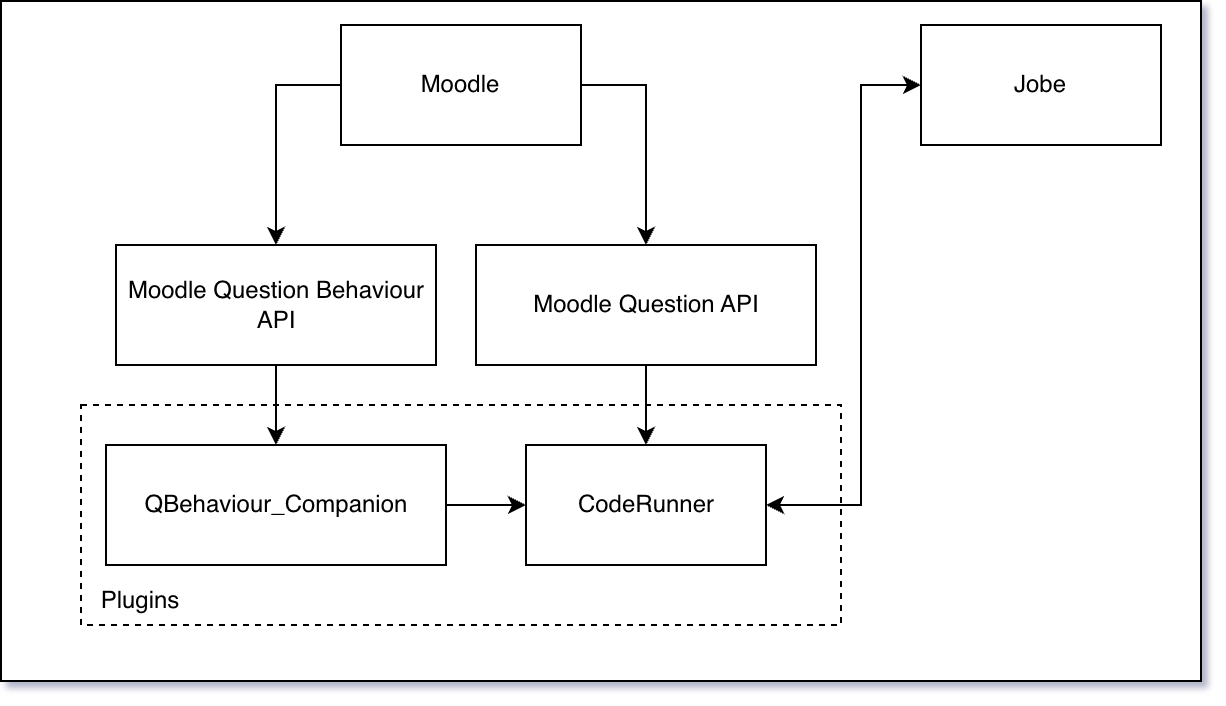
\includegraphics[width=0.8\textwidth]{figs/dependency_graph.png}
    \caption{Moodle \& Plugin dependency graph}
    \label{fig:dependency_graph}
\end{figure}

\subsubsection{Environment Setup}
After figuring out the project, the work turned to Docker: software that packages a program together with everything it needs into isolated `containers', so that the same setup runs identically on any machine~\cite{dockerjournal}. Due to a lack of knowledge, Docker had to be learned for the first time; however this allowed a much faster setup and an automatically repeatable environment.
This allowed Moodle to run, but not CodeRunner yet, because the in-development copies of the plugins had to be connected into the running Moodle (using Docker's bind mounts, which share a folder on the host machine with a container). This did not work as planned because the strict permissions of the macOS laptop used for development stopped the shared folders from working properly. Once this was realized, development switched to a desktop machine running Linux, which fixed the issue.
The project still did not work because Moodle's strict security policy blocks the web requests its components use to talk to one another (cURL requests), even local ones between Docker containers. Allowing these was required because one of the CodeRunner dependencies is Jobeinabox, the code-running server described above. This was not obvious at the time, and many hours were spent trying to figure out what was wrong with the Docker setup.

\subsubsection{Problem Identification}
The project was analysed by researching what issues CodeRunner has:
searching the public repository for posted issues, fielding a survey, interviewing lecturers, requesting fellow students' opinions, and including first-hand observations from using the system.
It quickly became clear that what had been presumed to be a lecturer problem was actually a software problem. User design books like Don Norman's \emph{The Design of Everyday Things}~\cite{designofeveryday} show that user error often isn't the user's fault. In the case of CodeRunner this was and still is absolutely correct. CodeRunner is one of the many software tools that will forever need to evolve due to the growing requirements of education~\cite{pieterse2013automated}.

\subsubsection{Review of the Author Page}
The existing design for both student facing and author facing pages was reviewed against the design literature introduced in Section~\ref{backg}: Don Norman~\cite{designofeveryday} and \emph{Don't Make Me Think} by Steve Krug~\cite{dontmakemethink} for the interfaces themselves, and Google's developer documentation style guide~\cite{googledevstyle} as the yardstick for the written documentation. 

The author page explains the frustration felt towards lecturers: the user experience provides a full suite of tools with no instructions on how to use them properly. A long single page document can be found on the CodeRunner documentation \cite{coderunnergitiodocs}, and it is extremely well-written and complete; however, it falls short of Google's guidance, which asks writers to organise content around the reader's task, to keep pages short and scannable, and to avoid explaining more than the task at hand requires. The CodeRunner manual does the opposite on each count: it is organised around the system's features, lives on one enormous page, and explains far more than the basic user needs. It is as though IKEA sent you a wardrobe with instructions on how to build every single type of wardrobe in their catalog and it is up to you to figure out which instructions you need to follow. This assessment directly shaped the documentation requirement (NFR3) and the task-focused documentation page later built to satisfy it.

\begin{figure}[h]
    \centering
    \setlength{\fboxsep}{0pt}%
    \fbox{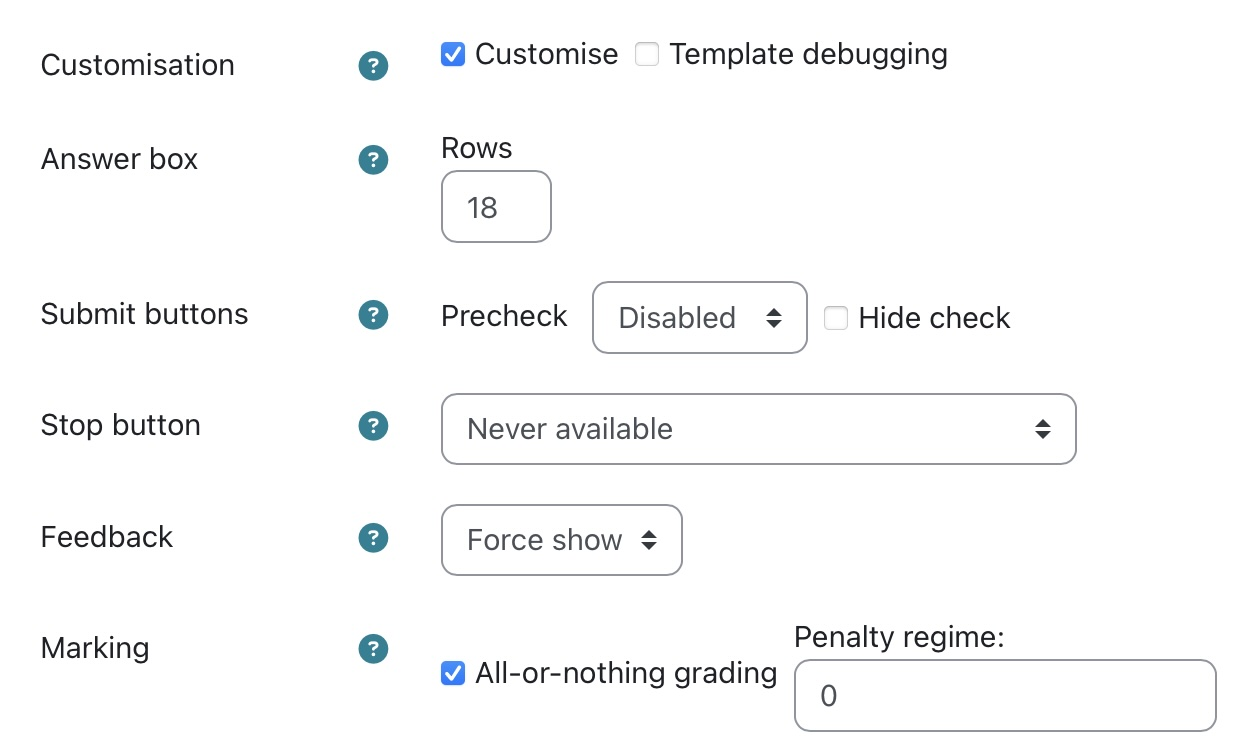
\includegraphics[width=\dimexpr\linewidth-2\fboxrule\relax]{figs/authorpage_1.jpg}}
    \caption{The CodeRunner author page's question-option controls, showing the per-label help buttons and the inconsistent label alignment discussed in this section.}
    \label{fig:authorpage_1}
\end{figure}

The author page (Figure~\ref{fig:authorpage_1}) is rough around the edges, and the burrs show on test cases: you can only add 3 test cases per request, no more no less. You also can't delete the excess test cases. The user interface as a whole is also very dense, jumbled and indecisive; some labels appear above their selectors, some appear to the left of them. Checkboxes scattered across the page, misaligned with their labels also. The corners of the test case boxes are also completely square, unlike every other box on the page, which are all rounded. Every help button beside every major label does nothing aside from opening one large column of text that explains what the feature does, but it disappears the moment you click elsewhere, and the text is difficult to read properly because it can overflow due to length (Figure~\ref{fig:authorpage_helpoverflow}). 

\begin{figure}[H]
    \centering
    \setlength{\fboxsep}{0pt}%
    \fbox{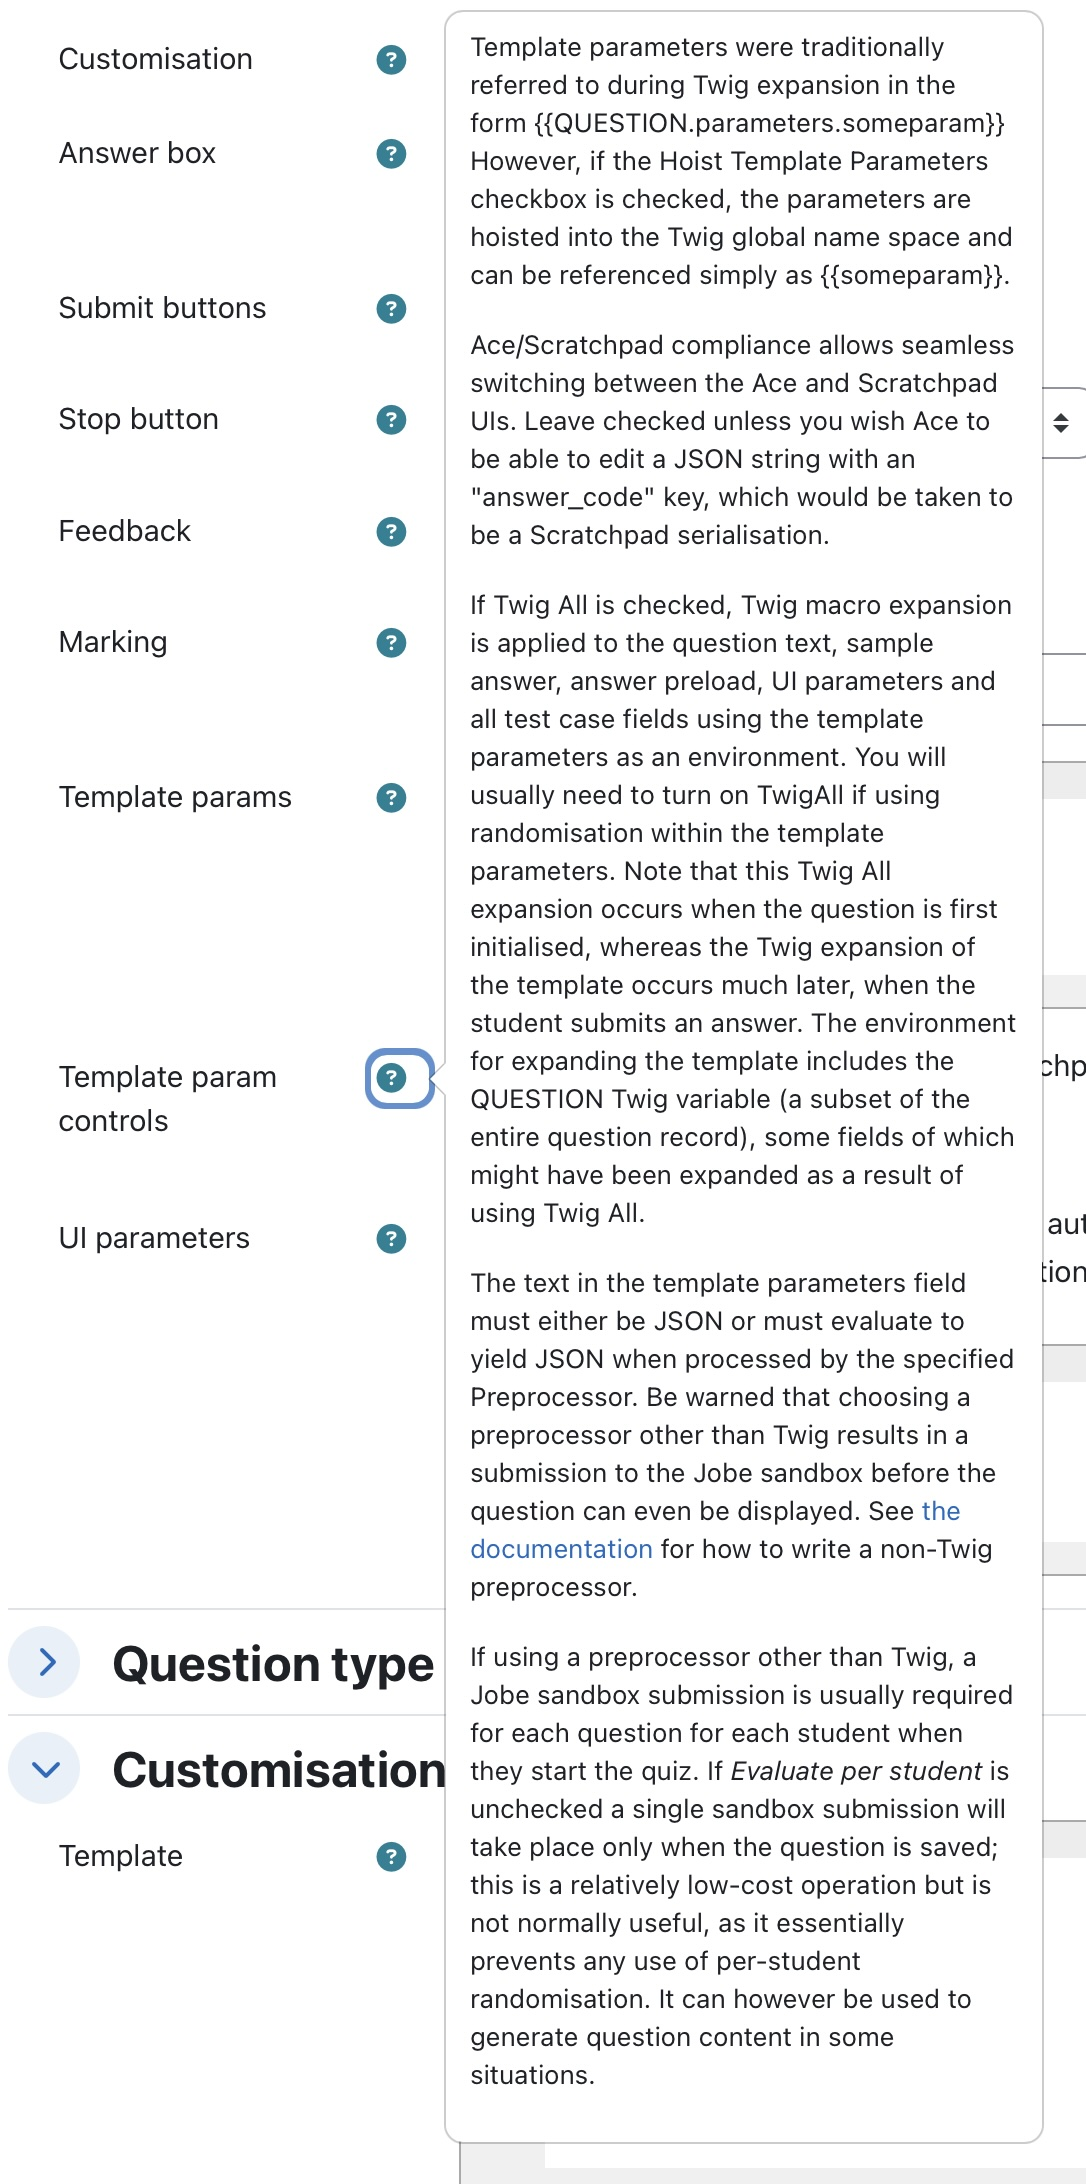
\includegraphics[height=0.55\textheight]{figs/authorpage_helpoverflow.jpg}}
    \caption{Author page showing the almost overflowing help hint discussed.}
    \label{fig:authorpage_helpoverflow}
\end{figure}

When the Precheck option is enabled, it appears in the label column of the test case instead of the input column to its right, and the padding of the row above separates it visually from the test case box it belongs to, appearing disjointed. A Lighthouse audit (an automated page-quality check built into the Chrome browser) scores this page at only 93\% for accessibility, a measure of how usable a page is for people relying on assistive tools such as screen readers, instead of the preferable 100\%: several of the input controls in CodeRunner lack ARIA labels (invisible text that a screen reader speaks aloud), as does the Ace Editor, the code-editing box embedded in the page. Despite the author page being very technically heavy, there are very few self-explanatory options; the help buttons make some of them self-evident, but they often fail to explain how the question lifecycle really works \cite{dontmakemethink}.

\subsubsection{Review of the Student Page}
The student-facing question answer page is polished and complete. This page is quite good when the author writes the questions correctly; for example, a bad question would be where the question description is too massive to view both the description and the answer box at once. Another example is when the author chooses to use hidden test cases (tests whose details are concealed from the student, so that answers cannot simply be written to pass them): this is good for the author but it does not help the student at all. Often an author will have many hidden test cases and it is unknown which one the student failed, especially under complex questions. Inspection of the code showed that a written answer in the page is only saved automatically every 60 seconds, in the background; while this is acceptable, the user might benefit from an affordance (in Don Norman's sense~\cite{designofeveryday}, a control that visibly invites its use) which allows them to save manually.

\subsubsection{Survey Analysis}

Furthermore, pursuing a survey, designed with reference to established principles of survey research~\cite{designingsurvey}, yielded further requirements and analysis. A list of comments and suggestions follows:
\begin{itemize} 
  \item `I don't like that hidden test cases don't tell the user where they went wrong', paraphrased, in reference to student-facing page, the system currently does not tell the student why they failed a hidden test case within a question.
  \item `A hint option that deducts marks if used' in reference to the student-facing page, the system should allow the user to get hints in exchange for a reduced mark.
    This option is very similar to giving hints on hidden test cases failed instead of silently erroring out.
  \item `An LLM to check whether the answer is close enough may be beneficial as CodeRunner often expects unrealistically exact inputs/outputs.' in reference to the grading methods available.
  \item `An attached command terminal for outputs would be useful for interactive prototyping.' in reference to the student-facing page, it shall allow the user to run custom commands and tests.
  \item `It would be nice if it had LSP support.' in reference to the editor, the idea is to extend the editor's ability to flag errors and runtime errors prior to the answer being checked.
  \item `Provide commands such as the gcc line which could be copied into a clipboard' paraphrased, in reference to the student-facing page, the question should provide a codebox which allows the user to click a copy button instead of selecting and copying it manually.

\end{itemize}

In the order listed above, the following discusses the viability and benefit-to-cost ratio of each suggestion.

Providing a hint button is an idea very similar to allowing the user to get more information out of hidden test cases; the latter is arguably the bigger problem because in most cases the questions the lecturers write are well detailed and more than enough. The issue with hidden test cases is that often the student can be left guessing what is wrong instead of getting a detailed answer as to why they are failing, which costs them even more penalty if they guess wrong. In the real world, a developer can usually find a reason as to why something in their code isn't working correctly.

An LLM (large language model, the technology behind tools such as ChatGPT) addition to the question grading options is an interesting suggestion because it is a genuinely good solution in low-complexity questions, but in higher complexity questions this method can give different grades to the same answer across two different cases. It is therefore unreliable, rolling the dice with each grade, and it leaves the author susceptible to scrutiny; recent benchmarking still places even state-of-the-art models behind human tutors at grading tasks~\cite{llmgrading}. The level of complexity to implement such a feature isn't the problem because you can create something similar to Jobe or extend Jobe, however there is almost no university with enough money or hardware to run LLMs for grading at full capacity.

An interactive terminal included in a question is an appealing idea, however the complexity of implementing such an element is far beyond the scope of the project. To implement this, the system requires a host which is able to expose 100 or more simultaneous containers for use, as well as websocket connections. It would most likely act like SSH, however written in JS, the problem with this is that rewriting SSH in JS would prove incredibly time consuming and a security nightmare.

The Language Server Protocol (LSP) implemented into the Ace editor is a great idea; several contributors have managed to write a package, \texttt{ace-linters}, which does this exact thing. The trouble would most likely be controlling how to get fine control over the linter via PHP when the author does not want this feature enabled.

Providing a copy button inside codeblocks would be a good idea and possesses a high benefit-to-cost ratio.

\subsection{Requirements}
% Here you explain what the functional and non-functional requirements are. Explain how you prioritised them. 
%   See \url{https://www.nuclino.com/articles/functional-requirements} for more informatioqn. 
%
%    \textbf{Functional requirement:} "The system must \textbf{\emph{do}} [requirement]."
%
%     \textbf{Non-functional requirement:} "The system shall \textbf{\emph{be}} [requirement]."q
%
%
% Well-written functional requirements typically have the following characteristics:
% \begin{description}
%
%
%
%     \item[Necessary:] Although functional requirements may have different priority, every one of them needs to relate to a particular business goal or user requirement.
%
%   \item[Concise:] Use simple and easy-to-understand language without any unnecessary jargon to prevent confusion or misinterpretations.
%
%  \item[Attainable:] All requirements you include need to be realistic within the time and budget constraints set in the business requirements document.
%
%  \item[Granular:] Do not try to combine many requirements within one. The more precise and granular your requirements are, the easier it is to manage them.
%
%  \item[Consistent:] Make sure the requirements do not contradict each other and use consistent terminology.
%
%  \item[Verifiable:] It should be possible to determine whether the requirement has been met at the end of the project.
%     \end{description}
% TODO: assign MoSCoW priorities (Must/Should/Could) to each requirement.
\subsubsection{Development Environment Requirements}
\begin{itemize}
    \item[\textbf{DE1}] The environment must run Moodle, CodeRunner and its dependencies in isolation from the host machine. (Analysis)
    \item[\textbf{DE2}] The environment must be startable with a single command and produce a consistent, repeatable setup. (Analysis)
    \item[\textbf{DE3}] The environment must allow CodeRunner to be tested for regressions. (Analysis)
\end{itemize}

\subsubsection{System Functional Requirements}
\begin{itemize}
  \item[\textbf{FR1}] The author page must allow the author to delete test cases. (Analysis)
  \item[\textbf{FR2}] The author page must allow the author to add exactly the number of test cases they want. (Analysis)
  \item[\textbf{FR3}] The author page must keep help content visible until the author dismisses it. (Analysis)
  \item[\textbf{FR4}] The author page must render the Precheck option in its correct column, attached to its test case. (Analysis)
  \item[\textbf{FR5}] The author page must provide an option to give hints for hidden test cases. (Survey)
  \item[\textbf{FR6}] The student question page must allow the student to save their current work on demand. (Analysis)
  \item[\textbf{FR7}] The student question page must allow the student to manage the layout of the question. (GitHub Issue)
  \item[\textbf{FR8}] The student question page must allow the student to reclaim unused margin space to enlarge the question content area. (Analysis)
  \item[\textbf{FR9}] The student question page must provide a copy button on code blocks within the question text. (Survey)
\end{itemize}

\subsubsection{System Non-Functional Requirements}

\begin{itemize}
    \item[\textbf{NFR1}] The author page shall be visually consistent: uniform corner rounding, and labels and checkboxes aligned with their controls. (Analysis)
    \item[\textbf{NFR2}] The author page shall score at least 97\% on a Lighthouse accessibility audit, the maximum attainable given its third-party components. (Analysis)
    \item[\textbf{NFR3}] The documentation shall be effective and self-evident: task-focused and reachable directly from the question editing form. (Analysis)
\end{itemize}

The remaining survey suggestions (LSP support in the editor, an interactive terminal, and LLM-based grading) were considered and excluded from the requirements as out of scope; the reasoning is discussed in the Survey Analysis above.


\subsection{Design}
The elements and layout were designed using in-browser prototyping in place of wireframes. This method seemed best because the environment contained the most information, and recreating a wireframe within a graphic design tool seemed slower than using the DevTools environment. The other benefit was that CSS rules could be tested live and rapidly verified to work as intended. For each feature a layout and style were drafted, the design shown to peers and the supervisor for review, and only then committed to CSS and JS files.

\subsubsection{Interface Design}
The following interface designs for each element were tested via a survey and opinions requested over email.

The layout switcher found on the student-facing page is designed with a toggle to allow the student to choose between two interface layouts (Figure~\ref{fig:studentanswer_layouts}). It gives the user control over how the question is presented, which is usually a net positive for user experience.

\begin{figure}[H]
    \centering
    \setlength{\fboxsep}{0pt}%
    \begin{subfigure}{\linewidth}
        \centering
        \fbox{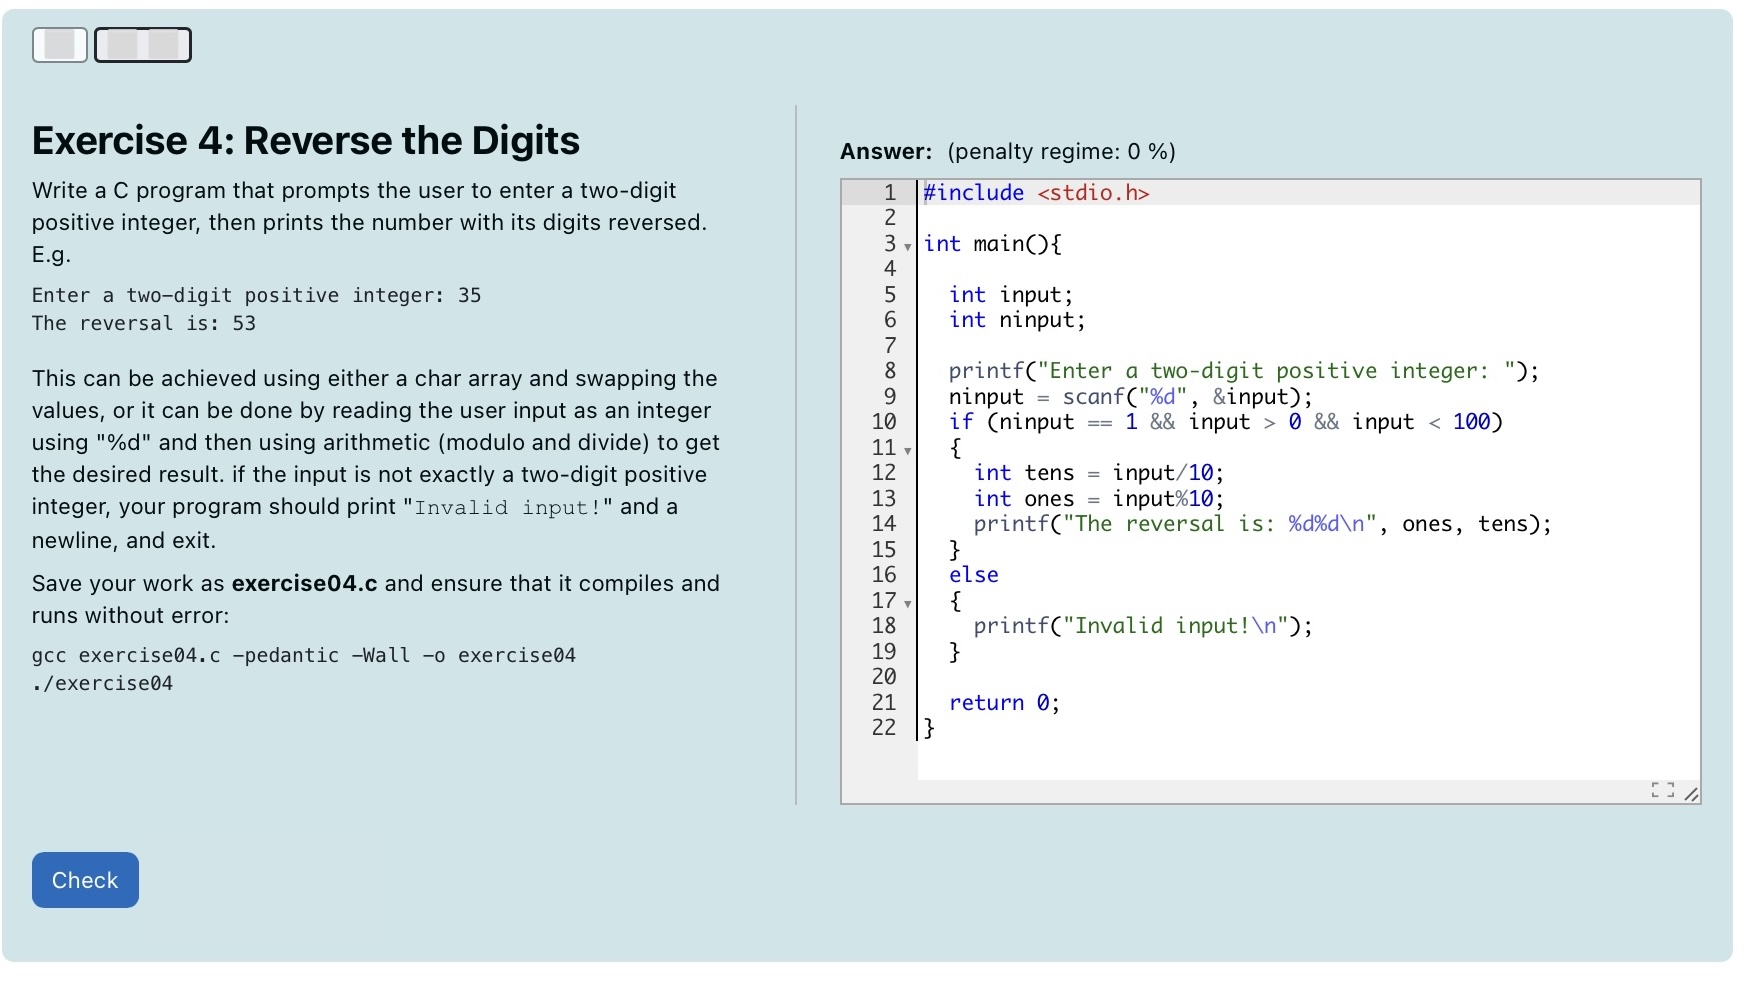
\includegraphics[width=0.72\linewidth]{figs/studentanswer_1.jpg}}
        \caption{Side-by-side view}
        \label{fig:studentanswer_sidebyside}
    \end{subfigure}

    \vspace{1em}
    \begin{subfigure}{\linewidth}
        \centering
        \fbox{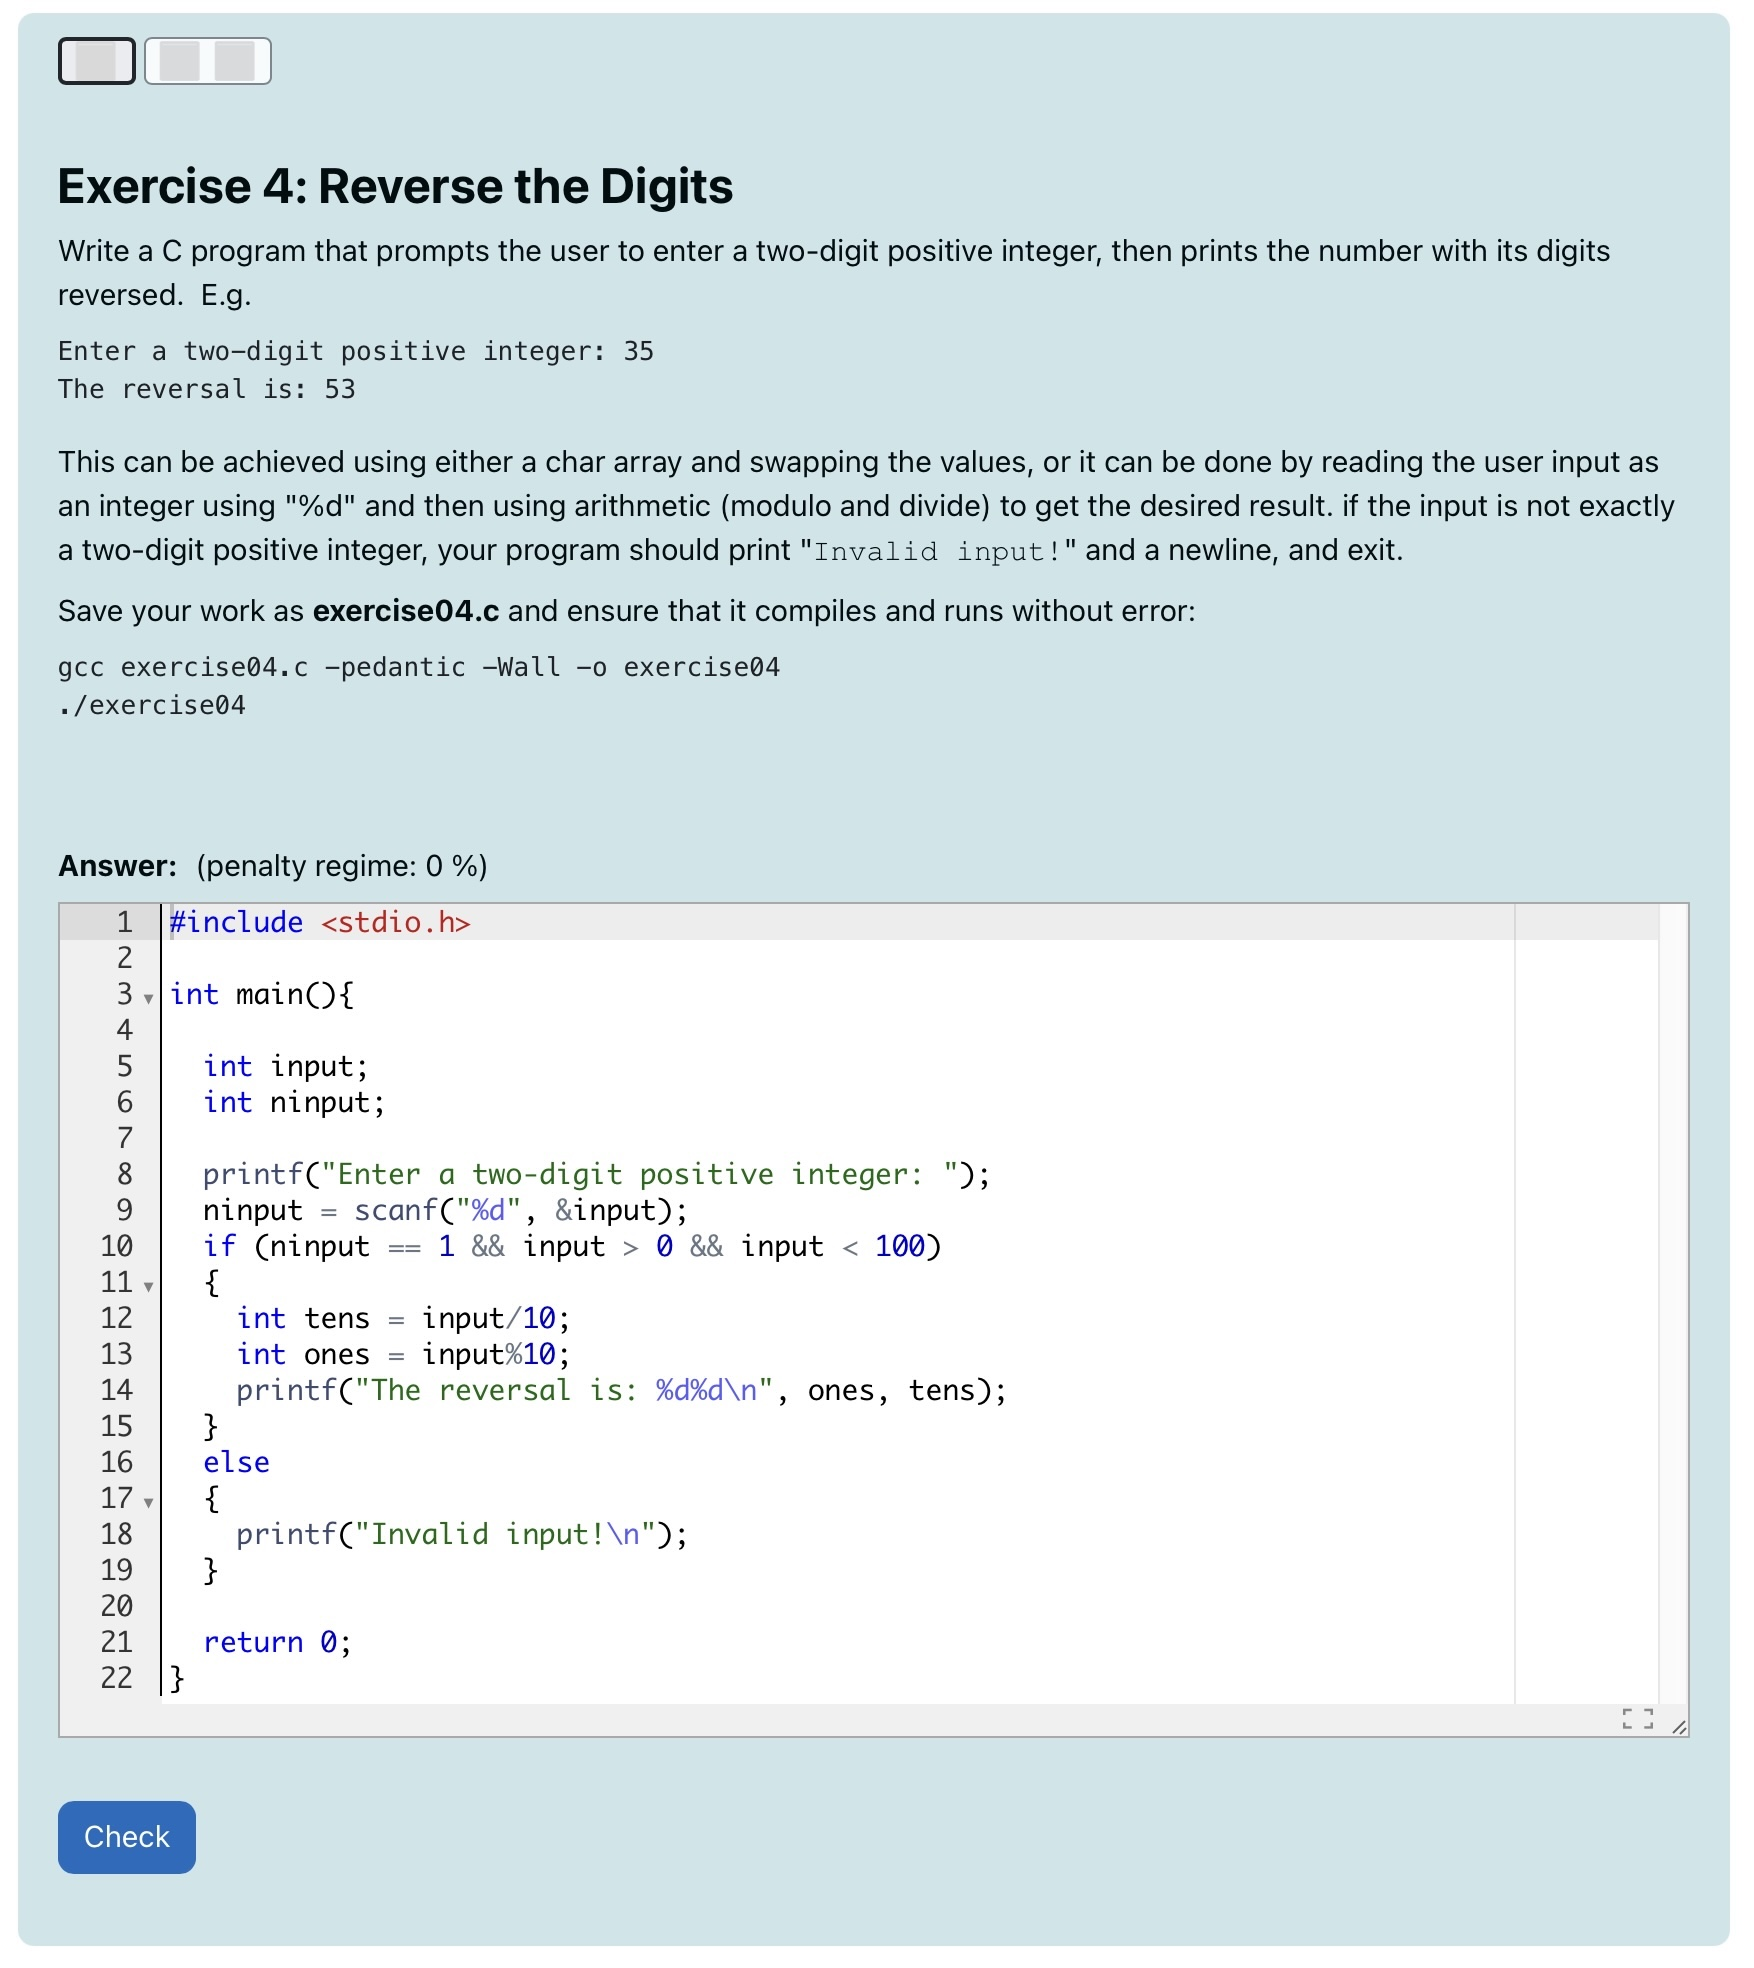
\includegraphics[width=0.6\linewidth]{figs/studentanswer_2.jpg}}
        \caption{Stacked view}
        \label{fig:studentanswer_stacked}
    \end{subfigure}
    \caption{The two student-facing question layouts offered by the layout switcher.}
    \label{fig:studentanswer_layouts}
\end{figure}

The Draft button found on the student-facing page was designed with the Bootstrap CSS framework in mind: Moodle itself uses Bootstrap at its core to style their interface, which allows existing button styles to be reused. With respect to the other existing buttons, the Draft button is styled as the lowest priority, the least attention-grabbing; the gray outlined button is barely noticeable until it is looked for: discoverable but not offensive to the eyes (Figure~\ref{fig:savedraft}).


\begin{figure}[H]
    \centering
    \setlength{\fboxsep}{0pt}%
    \begin{subfigure}[b]{0.48\textwidth}
        \centering
        \fbox{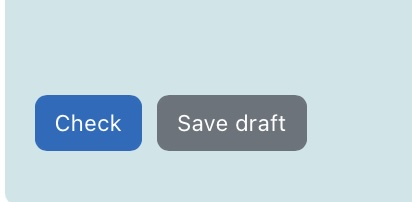
\includegraphics[height=2.5cm]{figs/coderunner-save-draft.jpg}}
        \caption{Hovered view}
        \label{fig:savedraft_hovered}
    \end{subfigure}
    \hfill
    \begin{subfigure}[b]{0.48\textwidth}
        \centering
        \fbox{
\includegraphics[height=2.5cm]{figs/savedraft.jpg}}
        \caption{Unhovered view}
        \label{fig:savedraft_unhovered}
    \end{subfigure}
    \caption{The Save Draft button, hovered and unhovered.}
    \label{fig:savedraft}
\end{figure}

The test cases found on the author page had their styles updated, and a new button was added for deleting test cases. This button also requires the user to confirm their choice using an alert dialog to prevent accidental work loss.

The info panel on the student-facing page was slightly reworked by the addition of a fold/float button. This button was originally designed to completely hide the info panel to allow the page to reduce its margins therefore allow the main content to consume more space for improved readability; however, experimenting with the panel revealed it already supported a different variant of this in the mobile version of the student-facing page. The in-place alternate style is leveraged by allowing the user to use a button to manually set the info panel into mobile mode.

The documentation page added by this project required almost zero interface design because of how the system is designed: the input for this page is entirely Markdown (MD), which lets the PHP MD parser take care of the element and CSS styling. The output is then rendered as HTML onto the page. The input is also a part of the interface because it is written in Markdown, which makes writing up-to-date documentation far more accessible and readable. To quote a survey response: `Currently the best way to learn CodeRunner is to have someone that knows it explain it to you.' Making the documentation accessible and easy to update means that it has the potential to be extended in the future by other contributors and CodeRunner question authors who are experts in it.

\subsubsection{System Design}

The following diagram describes the Docker topology designed for the development part of this project:

\begin{figure}[h]
    \centering
    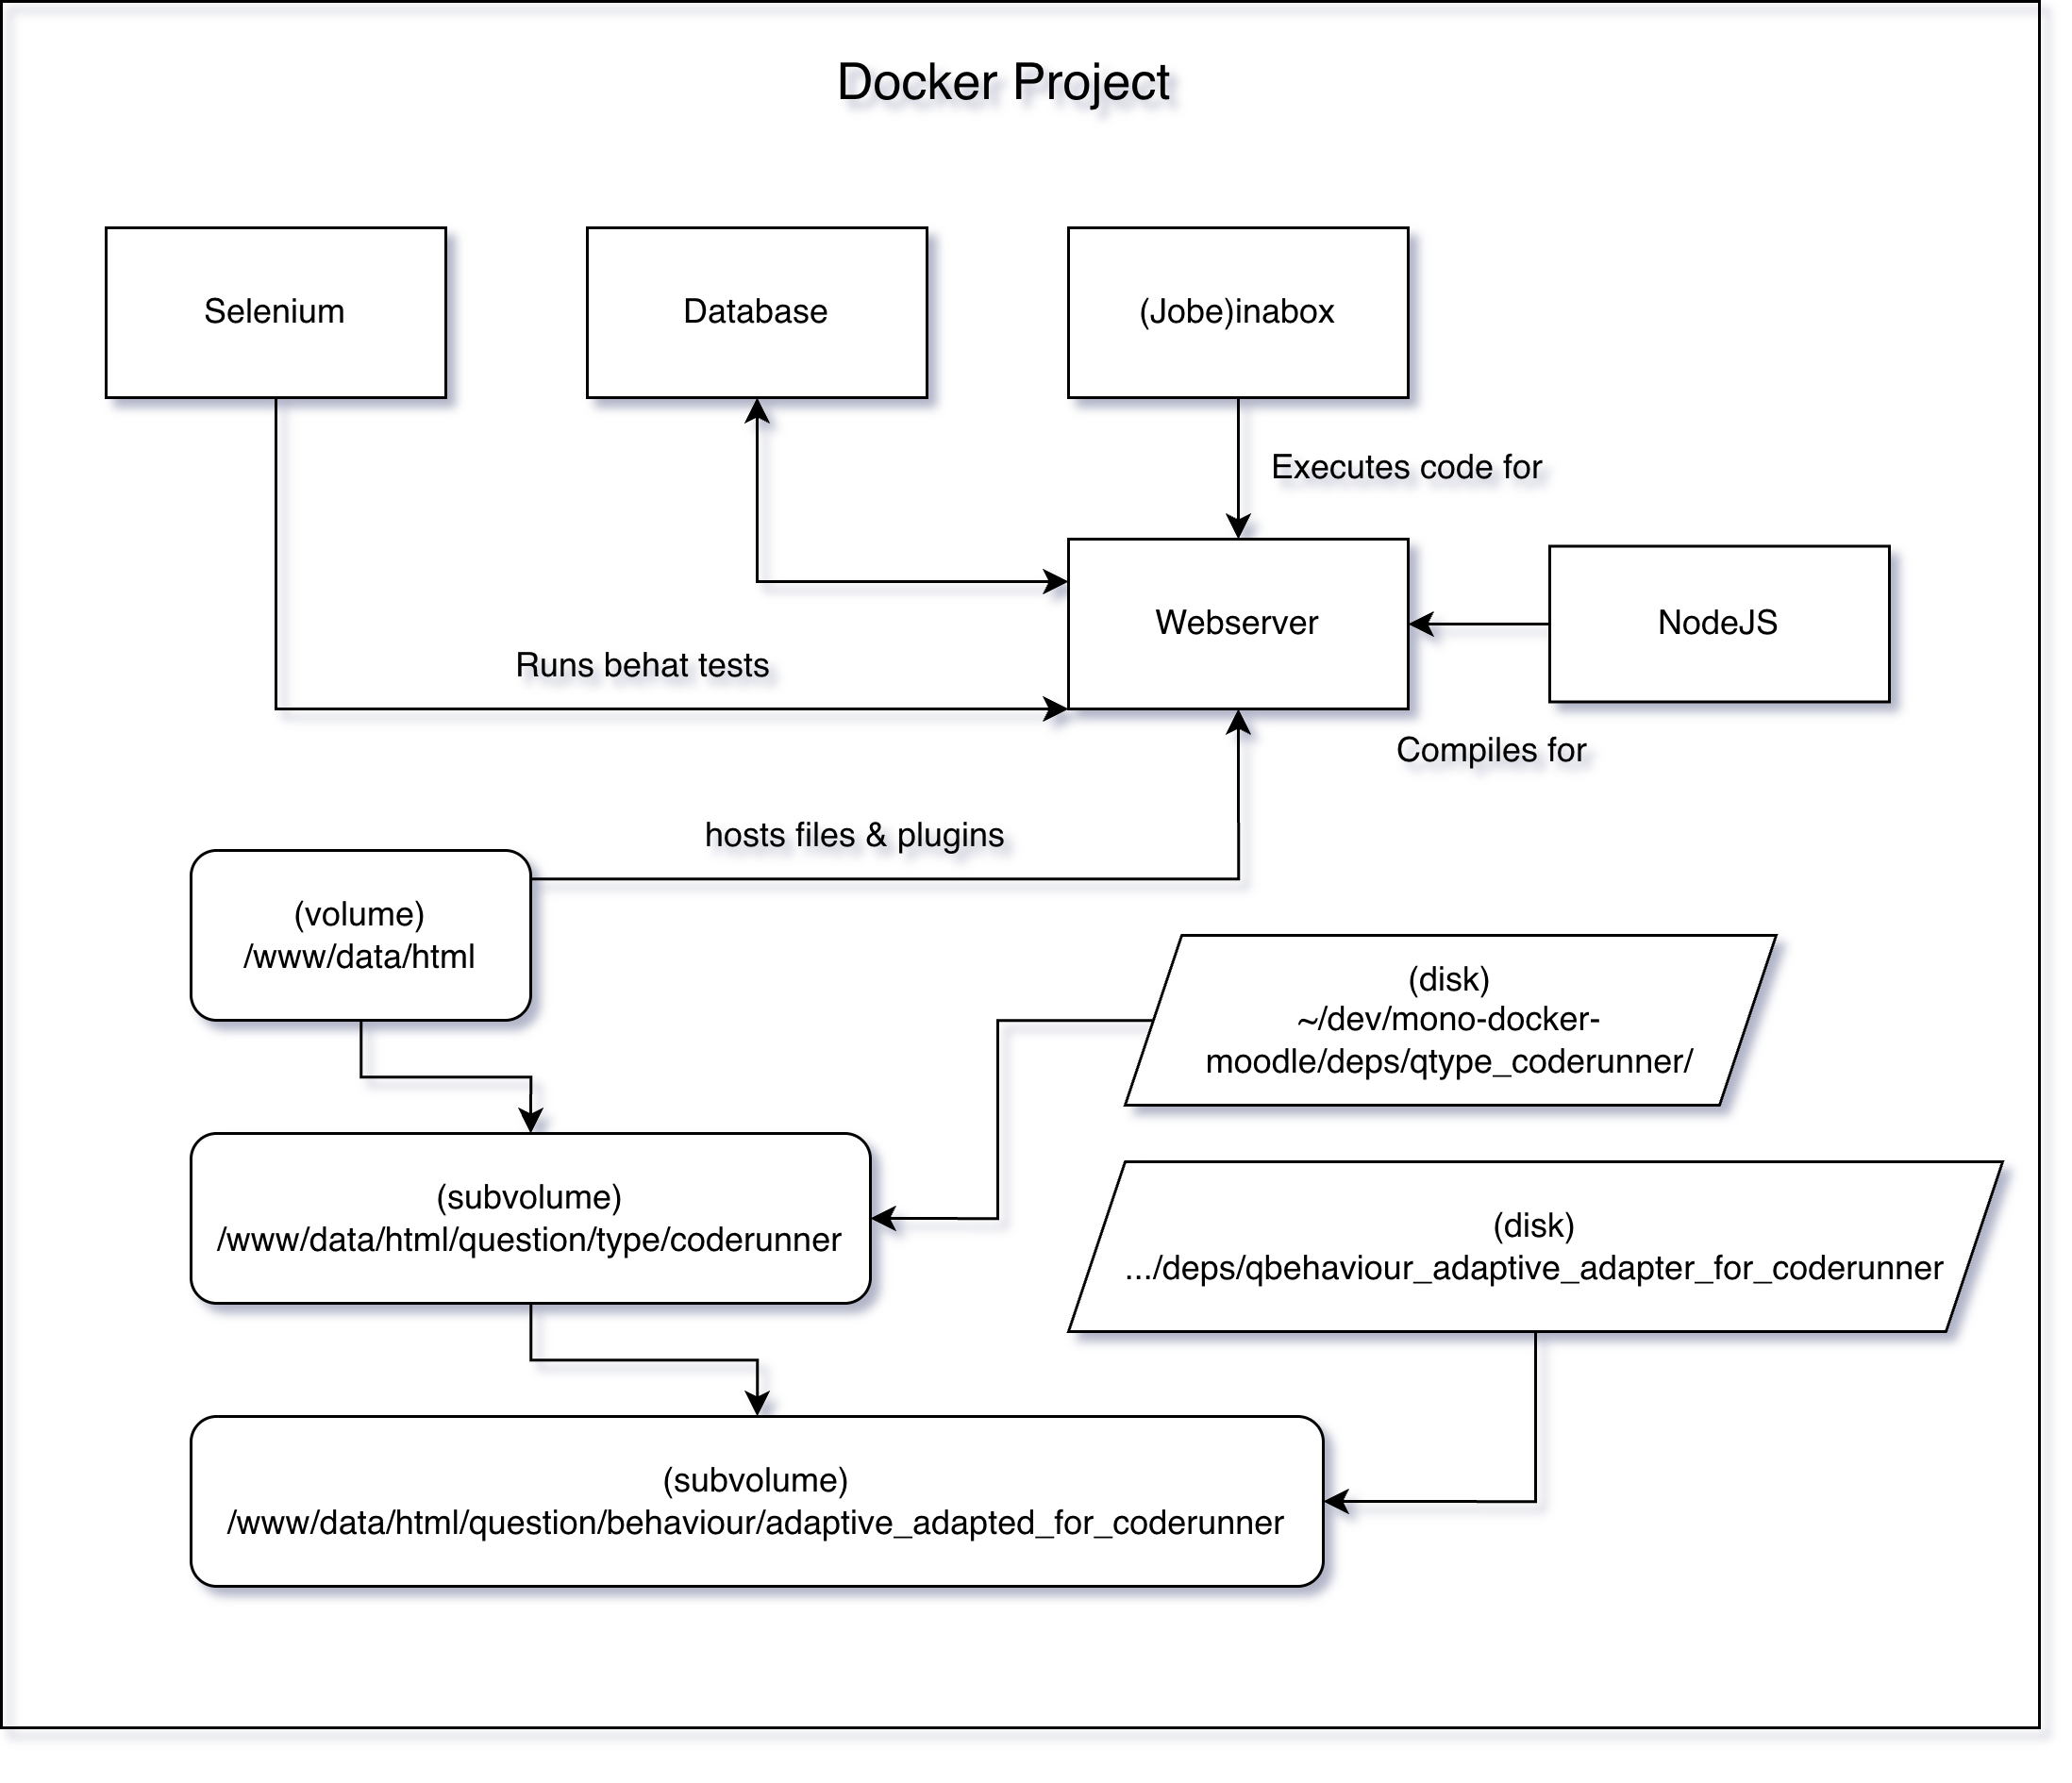
\includegraphics[width=0.8\textwidth]{figs/docker_project.png}
    \caption{Docker architecture}
    \label{fig:docker_project}
\end{figure}

The following diagram is in direct reference to the analysis and describes the sequence of how CodeRunner and Moodle interact to fulfil a question result.

% TODO: insert submission sequence diagram (student -> behaviour plugin -> question type -> Jobe -> result table).

To save the layout state and question info hidden state, a \texttt{sessionStorage} object is used. This allows the page to remember what layout each question was in, sparing the user the cognitive load of recognising what happened to their questions. The data structure avoids polluting \texttt{sessionStorage} with a separate entry per question by keeping all question states under a single key. The data structure in TypeScript goes as follows:
\lstset{
    frame=tb,                           % Frame at top and bottom
    language=Typescript-min,            % Choose the programming language
    basicstyle=\ttfamily\small,         % Use monospace font
    keywordstyle=\color{blue}\bfseries, % Style for language keywords
    commentstyle=\color{green!50!black},% Style for comments
    stringstyle=\color{orange},         % Style for strings
    numbers=left,                       % Line numbers on the left
    numberstyle=\small\color{gray},      % Style for line numbers
    breaklines=true,                    % Wrap long lines automatically
    tabsize=4                           % Set tab spaces
}
\begin{lstlisting}[caption={TypeScript definition for Layout \& Question Info state}]
type QuestionState = {layout: string, infoCollapsed: boolean};
type QuestionID = string;
type QuestionStateTracker = Record<QuestionID, QuestionState>;
// Instead of a new sessionStorage entry per question,
// all question states are stored under one key.

const STORAGE_KEY = 'coderunner_layout';
let state: QuestionStateTracker =
    JSON.parse(sessionStorage.getItem(STORAGE_KEY) || '{}');
let question = state[questionID];
let layout = question.layout;
let infoCollapsed = question.infoCollapsed;

\end{lstlisting}

In some circumstances where the default option is different from the user-chosen option, such as the alternate layout, the page may render with the default option (e.g. style rules), then a lazily loaded script changes it. This sequence happens within 500ms on a good machine, which appears janky and broken. To prevent this, a script was added to the main renderer for CodeRunner which is injected into the page and runs before the first paint, preventing the janky behaviour by overriding the defaults to be the user-chosen ones instead.

The test cases in general required a rework to support deleting test cases. Developing a delete test case button for the author page revealed that test cases were managed and accessed by a continuous index, which broke when deleting test cases in the middle of the array. The parts that interacted with the list of test cases were rewritten to access by key instead of array index. This introduced no regressions according to Behat, PHPUnit and manual testing, and allowed the delete test case button to work correctly.

The lack of a database design is a deliberate decision: \texttt{sessionStorage} was chosen because the changes live in the browser instead of the persistent database. This seemed the most appropriate and least time-costly method. Of all the many changes made, any touching the backend are exclusively stateless or required zero changes in database schema, therefore only browser data needed to be saved. From an end-user's perspective, such a feature would not be expected to save the layout across session resets.

